%%%%%%%%%%%%%%%%%%%%%%%%%%%%%%%%%%%%%%%%%%%%%%%%%%%%%%%%%%%%%%%%%%%%%%%%%%%%%%%
%%                                                                           %%
%%   Dr Varun Ojha                                                           %%
%%   Lecturer, Department of Computer Science                                %% 
%%   University of Reading, UK                                               %%
%%                                                                           %%
%%%%%%%%%%%%%%%%%%%%%%%%%%%%%%%%%%%%%%%%%%%%%%%%%%%%%%%%%%%%%%%%%%%%%%%%%%%%%%%
%%%%     SETTING STARTS - DO NOT CHANGE Unless your TeX setting require so   %%
%%%%%%%%%%%%%%%%%%%%%%%%%%%%%%%%%%%%%%%%%%%%%%%%%%%%%%%%%%%%%%%%%%%%%%%%%%%%%%%
%%----------------------------------------------------------------------------------
% DO NOT Change this. It is the required setting A4 page, 11pt, onside print, book style
%%----------------------------------------------------------------------------------
\documentclass[a4paper,11pt,oneside]{book}
\usepackage[italian]{babel}

%%-------------------------------------
%% Page margin settings - % half inch margin all sides (recommended)
%%-------------------------------------
\usepackage[margin=1.2in]{geometry} 

%%-------------------------------------
%% Font settings - % CM San or Ariel (recommended)
%%-------------------------------------
% Switch the following two line off: to revert back to default LaTex font (NOT recommended)
\usepackage{amsfonts}
\renewcommand*\familydefault{\sfdefault}

%%-------------------------------------
%% Math/Definition/Theorem/Algorithm packages settings 
%%-------------------------------------
\usepackage[cmex10]{amsmath}
\usepackage{amssymb}
\usepackage{amsthm}
\newtheorem{mydef}{Definition}
\newtheorem{mytherm}{Theorem}

%%-------------------------------------
%% Algorithms/Code Listing environment settings  - 
%% Please do not change these settings
%%-------------------------------------
\usepackage{algorithm}
\usepackage{algpseudocode}
\renewcommand{\algorithmicrequire}{\textbf{Input:}}
\renewcommand{\algorithmicensure}{\textbf{Output:}}
\usepackage[utf8]{inputenc}
\usepackage{listings}
\usepackage{xcolor}
\definecolor{codegreen}{rgb}{0,0.6,0.1}
\definecolor{codegray}{rgb}{0.5,0.5,0.5}
\definecolor{codeblue}{rgb}{0.10,0.00,1.00}
\definecolor{codepurple}{rgb}{0.58,0,0.82}
\definecolor{backcolour}{rgb}{1.0,1.0,1.0}

\lstdefinestyle{mystyle}{
    backgroundcolor=\color{backcolour},   
    commentstyle=\color{codegreen},
    keywordstyle=\color{codeblue},
    numberstyle=\tiny\color{codegray},
    stringstyle=\color{codepurple},
    basicstyle=\ttfamily\footnotesize,
    breakatwhitespace=false,         
    breaklines=true,                 
    captionpos=b,                        
    keepspaces=true,                 
    numbers=left,                    
    numbersep=5pt,                  
    showspaces=false,                
    showstringspaces=false,
    showtabs=false,                  
    tabsize=2,
    frame=none
}
\lstset{style=mystyle}

%%-------------------------------------
%% Graphics/Figures environment settings
%%-------------------------------------
\usepackage{graphicx}
\usepackage{subfigure}
\usepackage{caption}
\usepackage{lipsum}

%%-------------------------------------
%% Table environment settings
%%-------------------------------------
\usepackage{multirow}
\usepackage{rotating}
\usepackage{makecell}
\usepackage{booktabs}
\usepackage[normalem]{ulem}
\usepackage{adjustbox}
\useunder{\uline}{\ul}{}
%\usepackage{longtable,booktabs}

%%-------------------------------------
%% List of Abbreviations settings
%%-------------------------------------
\usepackage{enumitem}
\newlist{abbrv}{itemize}{1}
\setlist[abbrv,1]{label=,labelwidth=1in,align=parleft,itemsep=0.1\baselineskip,leftmargin=!}

%%-------------------------------------
%% Bibliography/References settings   - Harvard Style was used in this report
%%-------------------------------------
\usepackage[hidelinks]{hyperref}
\usepackage[comma,authoryear]{natbib}
\renewcommand{\bibname}{References} % DO NOT remove or switch of 

%%-------------------------------------
%% Appendix settings     
%%-------------------------------------
\usepackage[toc]{appendix}
%%%%%%%%%%%%%%%%%%%%%%%%%%%%%%%%%%%%%%%%%%%%%%%%%%%%%%%%%%%%%%%%%%%%%%%%%%%%%%%%%%%%%%%
%%%%                     SETTING ENDS                                            %%%%%%
%%%%%%%%%%%%%%%%%%%%%%%%%%%%%%%%%%%%%%%%%%%%%%%%%%%%%%%%%%%%%%%%%%%%%%%%%%%%%%%%%%%%%%%
\begin{document}

    \captionsetup[figure]{margin=1.5cm,font=small,name={Figure},labelsep=colon}
    \captionsetup[table]{margin=1.5cm,font=small,name={Table},labelsep=colon}
    % \setlipsumdefault{1}
    
    \frontmatter
    
    \begin{titlepage}      
        \begin{center}
            % \includegraphics[width=3cm]{figures/uorlogo.png}\\[0.5cm]
            {\LARGE Software Process Engineering}\\[2cm]
			%{\color{blue} \rule{\textwidth}{1pt}}
			
			% -------------------------------
			% You need to edit some details here
			% -------------------------------  
            \linespread{1.2}\huge {
                %%%%%%%%%%%%%%%%%%%%%%%%%%%%
                %TODO: 1 TITLE of Your PROJECT 
                %%%%%%%%%%%%%%%%%%%%%%%%%%%%
                % chnage the following line                
                Maraffa Online
            
            }
            \linespread{1}~\\[2cm]
			%{\color{blue} \rule{\textwidth}{1pt}}
            {\Large 
                %%%%%%%%%%%%%%%%%%%%%%%%%%%%
                %TODO: 2 YOUR NAME
                %%%%%%%%%%%%%%%%%%%%%%%%%%%%             
                % chnage the following line
                Sofia Tosi, Matteo Santoro
                % change end             
            }\\[1cm] 
            

            
    		% PLEASE DO NOT CHANGE THIS TEXT %
            %\large A report submitted in partial fulfilment of the requirements of\\the University of Reading for the degree of\\ Bachelor of Science in \textit{Computer Science}\\[0.3cm] 
            \vfill
            
            
            \today % Please update this date you can use \date{April 2020} for fixed date
        \end{center}
    \end{titlepage}
       
    
    % -------------------------------------------------------------------
    % Contents, list of figures, list of tables
    % -------------------------------------------------------------------
    
    \tableofcontents
    \listoffigures
    \listoftables
    \section{List of Abbreviations}
\chaptermark{List of Abbreviations}
%%%%%%%%%%%%%%%%%%%%%%%%%%%%%%%%%%%
%%  Enter your list of Abbreviation and Symbols in this file
%%%%%%%%%%%%%%%%%%%%%%%%%%%%%%%%%%%
\begin{abbrv}
    
    \item[SMPCS]			School of Mathematical, Physical and Computational Sciences
    
\end{abbrv}
 %  Enter your list of Abbreviation and Symbols in this file
    
    %%%%%%%%%%%%%%%%%%%%%%%%%%%%%%%%%%%%%%%%%%%%%%%%%%%%%%%%%%%%%%%%%%%%%%%%
    %%                                                                    %%  
    %%  Main chapters and sections of your project                        %%  
    %%  Everything from here on needs updates in your own words and works %%
    %%                                                                    %%
    %%%%%%%%%%%%%%%%%%%%%%%%%%%%%%%%%%%%%%%%%%%%%%%%%%%%%%%%%%%%%%%%%%%%%%%%
    \mainmatter
    % Read for preparation of document in LaTex 
    % Lamport, L. (1986), LATEX: A Document Preparation System, Addison-Wesley.
    
    \chapter{Introduction}
\label{ch:into} % This how you label a chapter and the key (e.g., ch:into) will be used to refer this chapter ``Introduction'' later in the report. 
% the key ``ch:into'' can be used with command \ref{ch:intor} to refere this Chapter.
MaraffaOnline è un'applicazione che permette alle persone di giocare al gioco di carte \href{https://it.wikipedia.org/wiki/Marafone_Beccacino}{Maraffa/Beccacino}. 
Il progetto consiste nell’eseguire una manutenzione evolutiva del gioco di carte reperibile su MaraffaOnline, attualmente sviluppato dalla prof.ssa Lumini.
In particolare la nuova versione avrà un'architettura a microservizi e introdurrà anche nuove funzionalità come formazione personalizzata delle squadre, una nuova modalità 
di gioco (vittoria 11 a 0 in caso di violazione delle regole da parte di una squadra), salvataggio delle statistiche delle partite e degli utenti, ...
\\
Per lo sviluppo è stato seguito un approccio Domain Driven Design, per il quale si è approfondito il dominio del gioco.
\\
È stata posta particolare attenzione alle tecniche di continuos integration, alle quali è stato dedicato uno dei capitoli di questo report.

% Meeting people in real life to challenge them in games can be sometimes difficult, especially when someone moves into a different city or a new disease force us to stay at home. 
% MaraffaOnline is a card game that allow players from different location to play together spending their time. Users can meet, create a game and play their cards using only allowed word and have some fun!
% The project consists of carrying out an evolutionary maintenance of the card game [Maraffa/Beccacino](https://it.wikipedia.org/wiki/Marafone_Beccacino) available on [MaraffaOnline](https://www.maraffaonline.it/), currently developed by Prof. Lumini. There is actually  a frontend in Angular, a basic API in C# and the user management is absent. Our work will be to add new functionalities and perform refactoring not only at the code level, but also at the architectural level.



    \chapter{Domain Driven Design}
\label{ch:ddd} %Label of the chapter lit rev. The key ``ch:lit_rev'' can be used with command \ref{ch:lit_rev} to refer this Chapter.

\section{Knowledge session for the exploration of the problem space}
\section{Ubiquitos Language}
**insert the dictionary**
\section{Bounded Context}
\section{Requisiti e casi d'uso}
\subsection{Requirments}
\subsection{Casi d'uso}
\section{Riflessioni}
**Spiegare per quale motivo i pattern del DDD non sono stati applicati**
(shared kernel, publish consumer, ...)
% https://guides.library.bloomu.edu/litreview
    % replace all text with your own text.
% in this template few examples are mention
\chapter{Implementation}
\label{ch:implementation} % Label for method chapter
% \section{Implementation}

% \section{TASK.REGISTRY?????}



\section{Componenti}

\subsection{Servizi di Business Logic e User Service}

Entrambi questi servizi sono stati realizzati con lo stack NestJS, un framework per Node.js che semplifica la realizzazione di web server e API REST.
Si occupano rispettivamente di gestire la logica di gioco e la gestione degli utenti che vogliono utilizzare il sistema, due core business del progetto.

\subsubsection{Business Logic}

Questo servizio mantiene al proprio interno tutte le regole del gioco e il calcolo dei punteggi. 
Ha svariati endpoint che permettono al middleware di avere il minor numero possibile di responsabilità, delegando al servizio di business logic le operazioni riguardanti il gioco.

Questa scelta è stata fatta per mantenere il middleware il più leggero possibile e per evitare che si occupi di operazioni non di sua competenza. Inoltre, in futuro sarà possibile aggiungere nuovi giochi modificando il meno possibile il middleware, che dovrà semplicemente occuparsi della gestione delle partite e comunicare tempestivamente con i servizi di business logic in base al gioco scelto.

\subsubsection{User Service}

Questo servizio gestisce gli utenti, quindi la loro registrazione, autenticazione e gestione dei dati personali.
Anche in questo caso, il middleware delega al servizio di gestione degli utenti le operazioni riguardanti gli utenti, per mantenere il middleware il più leggero possibile e per evitare che si occupi di operazioni non di sua competenza.
Il core di questo servizio è dato dalla combinazione di NestJS e TypeORM, che permettono di gestire in modo semplice e veloce la persistenza dei dati e le operazioni CRUD su un database MySQL.
Oltre alle informazioni degli utenti, il database contiene anche le informazioni riguardanti le partite giocate e le statistiche personali di ogni utente del sistema.

\subsection{Front-End}

Il front-end è stato realizzato con Angular e si occupa di gestire l'interfaccia grafica e la comunicazione con il middleware. 
Il progetto pilota di questo frontend è un template di una generica app in angular, questo velocizzato in parte fornendo una struttura e alcune best practice di angular di cui non si era a conoscenza. 
Sono state realizzate diverse pagine, tra cui la home page, la pagina di registrazione, la pagina di login, la pagina di gioco e la pagina di profilo utente.
Utilizza API REST per comunicare con il middleware e ottenere i dati necessari per il funzionamento del gioco, mentre utilizza WebSockets per la comunicazione in tempo reale con il middleware. 

%TODO altro da dire sui servizi ?

\subsection{Middleware}


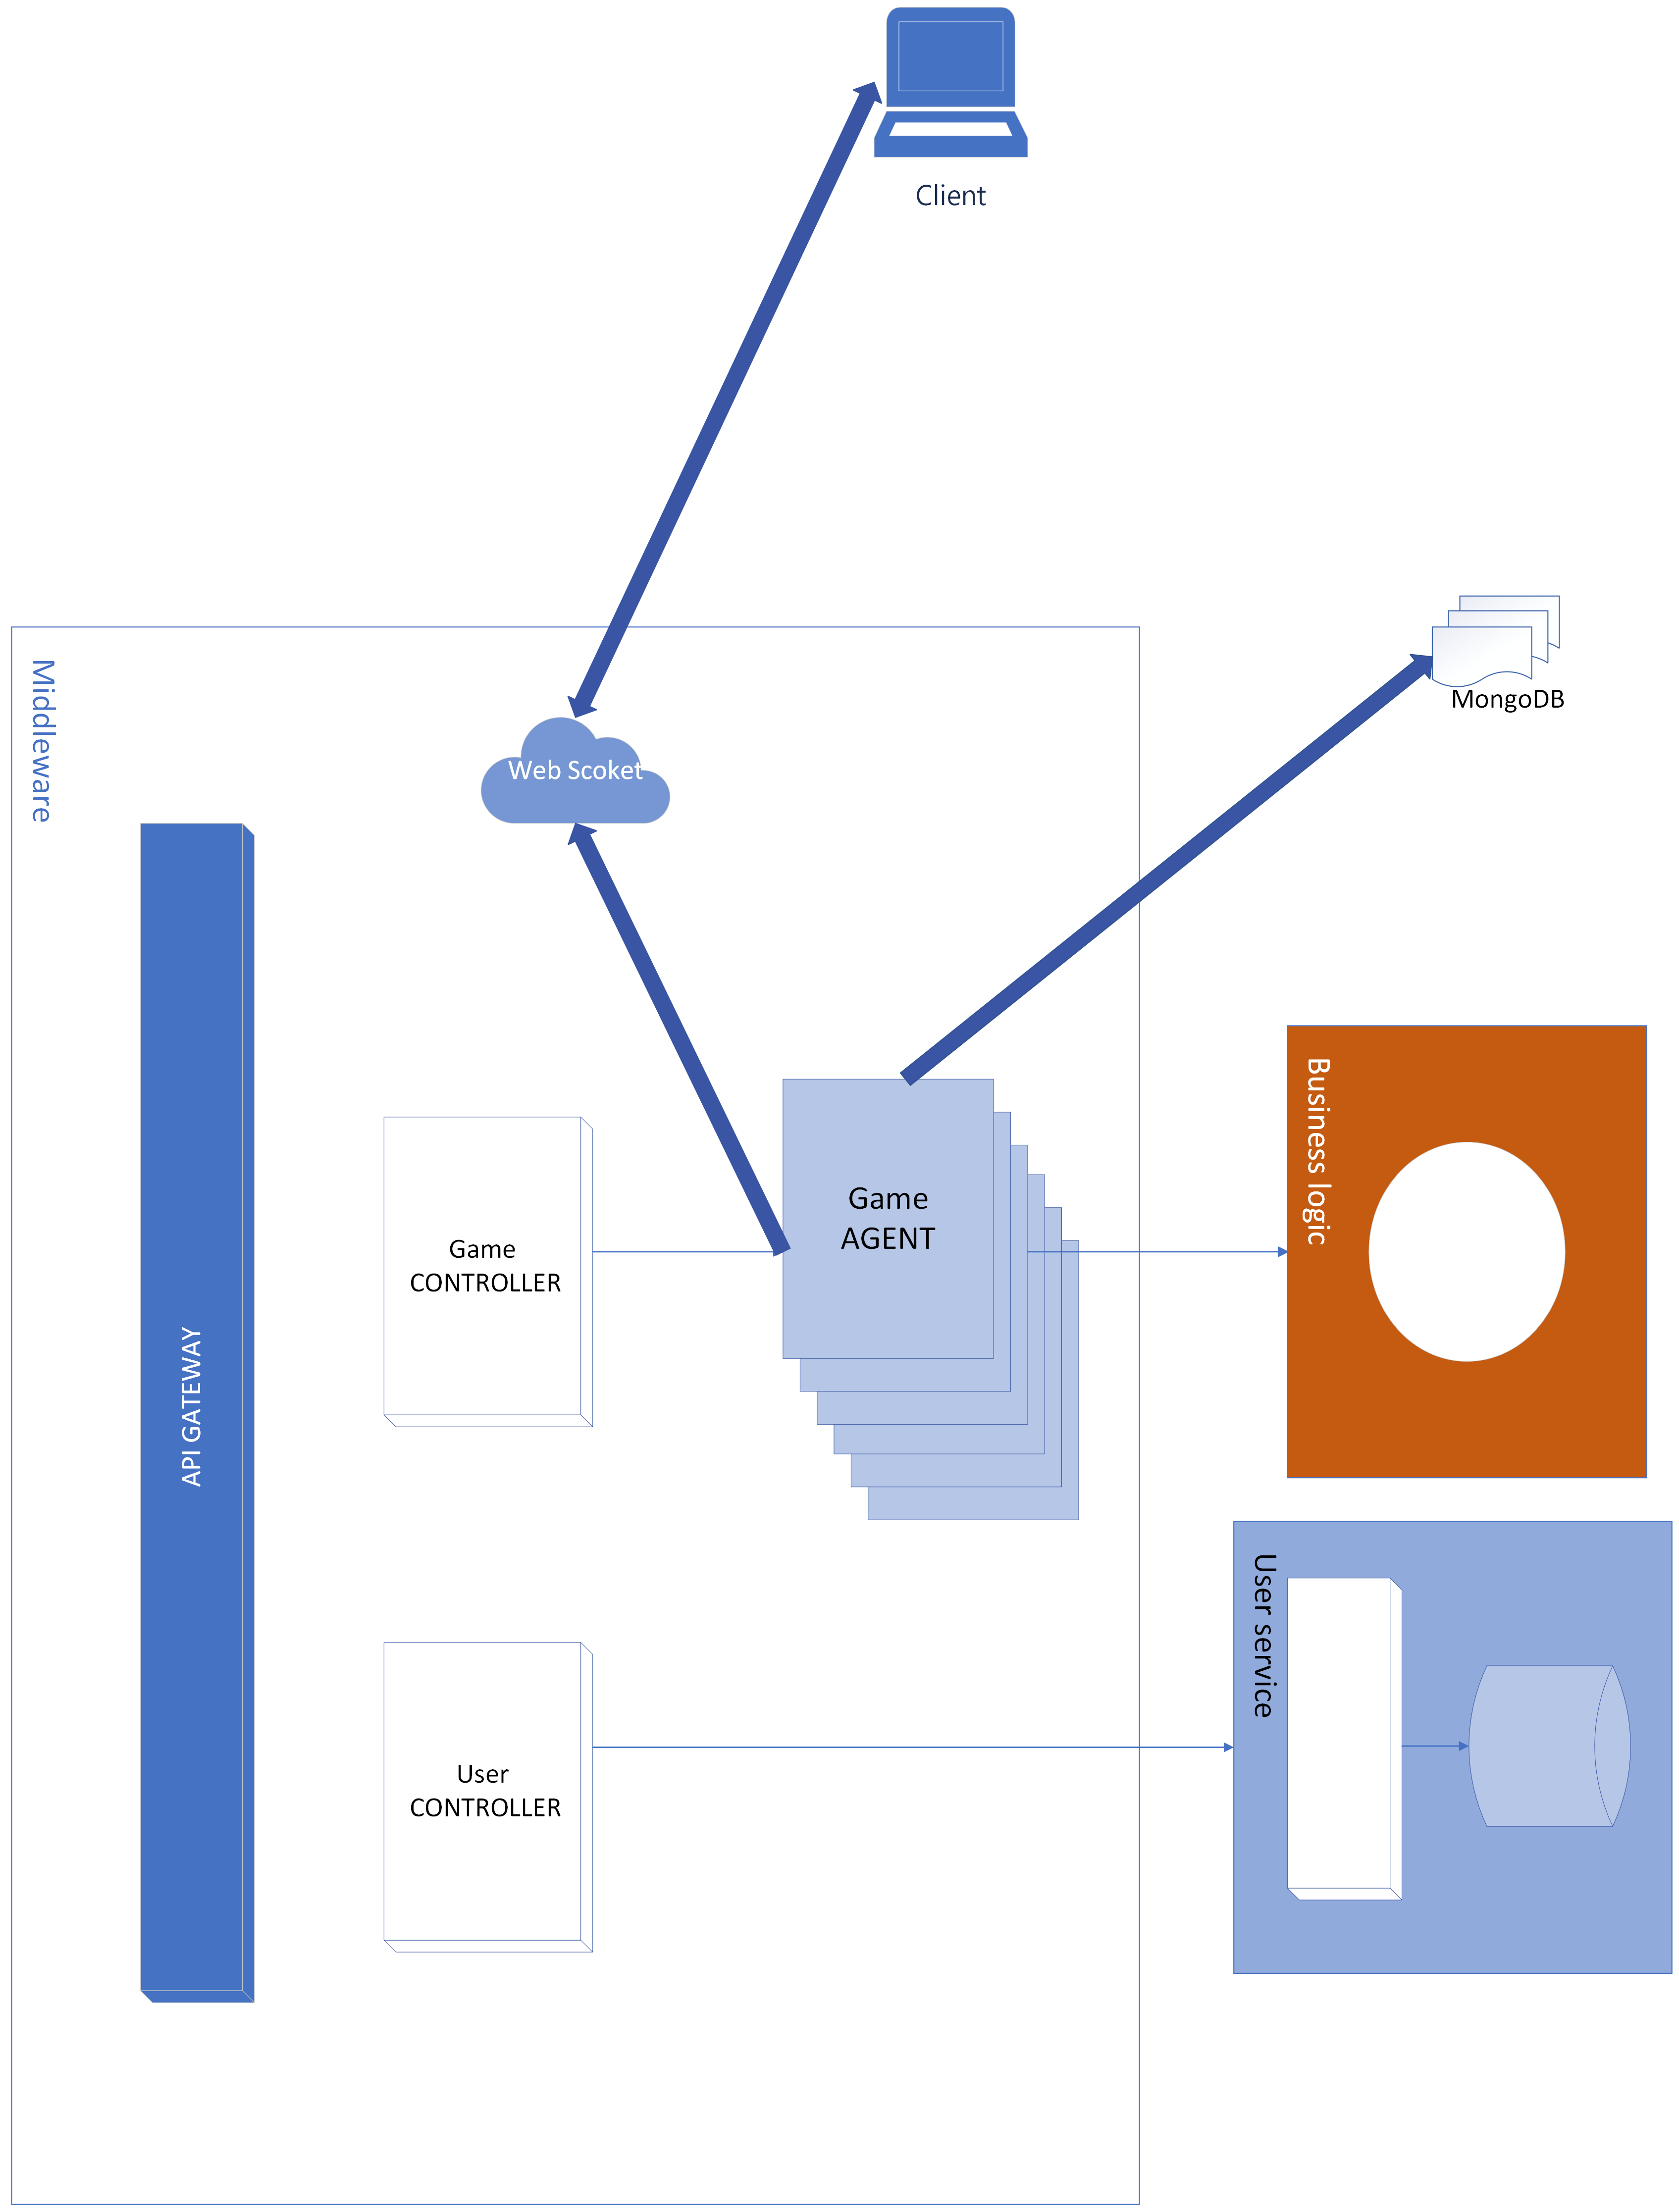
\includegraphics[width=12cm]{report/img/middleware.png}\\[10.5cm]

Come già citato, il middleware è il cuore del sistema. L'architettura utilizzata per la gestione delle partite è quella di un multi-agente, in cui ogni agente si occupa di gestire una partita 
e di orchestrare la comunicazione con gli altri servizi, come ad esempio il front-end. Questo core è stato realizzato con Vertx, che è stato utilizzato anche per creare un web-server in Java.

Inoltre, al middleware è collegato un database NoSQL su MongoDB, che viene aggiornato a ogni trick completato dai giocatori per creare uno storico delle partite e salvare le loro decisioni in gioco. 
Questa raccolta di dati sarà parte di uno sviluppo futuro, in cui, dopo aver raccolto una grande quantità di dati di partite, si potrà tentare di creare un modello di machine learning per sviluppare un'intelligenza artificiale che possa giocare al posto di un giocatore umano.



\section{Tecnologie}
% (-swagger, -postman, autogenerazione javadoc?, JWT per autenticazione utenti,
%  docker, nodejs, typescript, mongodb, jest, angular, figma, ...)
\subsection{Swagger - OpenAPI}

Uno dei requisiti fondamentali di questo progetto è stata la documentazione delle API.
Per fare ciò è stato utilizzato Swagger, un framework open-source che permette di descrivere, produrre e consumare servizi web RESTful. 
Swagger permette di testare le API direttamente dalla documentazione, grazie a un'interfaccia grafica che consente di inviare richieste e visualizzare le risposte.

\vspace{1cm}

Per i servizi creati in Node.js è stata utilizzata una libreria ad hoc, in grado di generare la documentazione automaticamente tramite i corretti decoratori.
Al contrario, per i servizi in Java non esiste alcuna libreria in grado di generare automaticamente la documentazione API a partire dai metodi esposti, quindi è stata creata manualmente.
Grazie a un lavoro preliminare open-source svolto da \href{https://github.com/anupsaund}{\underline{Anup Saund}} sulla sua repository \href{https://github.com/anupsaund/vertx-auto-swagger}{\underline{Vertx auto swagger}}, è stato possibile creare automaticamente un file HTML contenente la documentazione delle API esposte dai servizi in Java. 
Purtroppo, questo file non era in grado di aggiornarsi automaticamente in caso di modifiche alle rotte, quindi è stato necessario adattarlo per renderlo più flessibile e adatto al nostro progetto.

\vspace{1cm}

Vertx è una libreria davvero completa e ben strutturata. È stato possibile creare un Router in grado di gestire tutte le rotte del progetto in Java utilizzando una semplice classe astratta che ha definito tutti i metodi utilizzati nel progetto, tramite la quale si è potuto razionalizzare il codice e creare dinamicamente la funzionalità richiesta.

\begin{lstlisting}[language=Java, caption={Semplice interfaccia per le rotte HTTP}, label=list:java_swagger_interface]
package httpRest;

import io.vertx.core.Handler;
import io.vertx.core.http.HttpMethod;
import io.vertx.ext.web.RoutingContext;

public interface IRouteResponse {
    HttpMethod getMethod();
    String getRoute();
    Handler<RoutingContext> getHandler();
}
\end{lstlisting}

La parte realmente complicata è stata fare in modo che le annotazioni presenti nel codice sorgente venissero lette e trasformate in un file JSON che rappresentasse correttamente la documentazione delle API. 
Dopo alcuni tentativi, è stato possibile automatizzare anche questa operazione.

\begin{lstlisting}[language=Java, caption={Aggiunta dei moduli delle classi contenenti rotte HTTP}, label=list:java_swagger_modules]
final ImmutableSet<ClassPath.ClassInfo> modelClasses = ImmutableSet.<ClassPath.ClassInfo>builder()
        .addAll(this.getClassesInPackage("game"))
        .addAll(this.getClassesInPackage("userModule"))
        .addAll(this.getClassesInPackage("BLManagement"))
        .addAll(this.getClassesInPackage("chatModule"))
        .build();
\end{lstlisting}

\vspace{1cm}

Java permette di creare oggetti molto complessi, diversi dai JSON / object solitamente utilizzati in JavaScript. Era fondamentale poter adoperare questi schemi per avere una documentazione ricca e per poter testare velocemente le API senza utilizzare necessariamente un client come Postman. 

Infine, per poter mostrare correttamente la documentazione, è stato necessario creare un file HTML che permettesse di visualizzare la documentazione in modo chiaro e ordinato. Questo file statico, presente nella repository del progetto, utilizza come fonte il file JSON di OpenAPI che viene rigenerato a ogni build del progetto, in modo da avere sempre la documentazione aggiornata.

\subsection{Postman}

Swagger ha semplificato lo sviluppo delle API e il loro funzionamento, ma non è sostenibile per testare chiamate API successive che seguono un certo ordine o che necessitano di payload specifici. Postman è stato fondamentale per risolvere questo problema.

È stata creata una raccolta di richieste, comodamente esportate da Swagger senza alcun bisogno di riscrittura. Queste possono contenere payload parametrizzati grazie alle variabili di ambiente settabili una volta per tutte, come ad esempio il GameID, che altrimenti, una volta creato, deve essere copiato e incollato in ogni richiesta successiva che lo richiede.

L'altro grande vantaggio di utilizzare Postman è stata la funzionalità Flows, che permette di creare un diagramma di flusso delle richieste e di salvare alcune risposte in variabili. Fino a quando non si è arrivati ad avere un frontend funzionante, questi Flows sono stati utili per trovare eventuali bug e avere ben chiaro il flusso di chiamate che sarebbero dovute essere implementate nel frontend, il che ha velocizzato lo sviluppo del frontend, seppur in minima parte.

E' stato realizzato un flow che simulasse la creazione di una partita, l'iscrizione di 4 giocatori, l'avvio della partita e la simulazione di un turno completo di gioco. Questo ha permesso di testare in modo spedito molte delle funzionalità del sistema, e di trovare eventuali bug in modo altrettanto rapido.

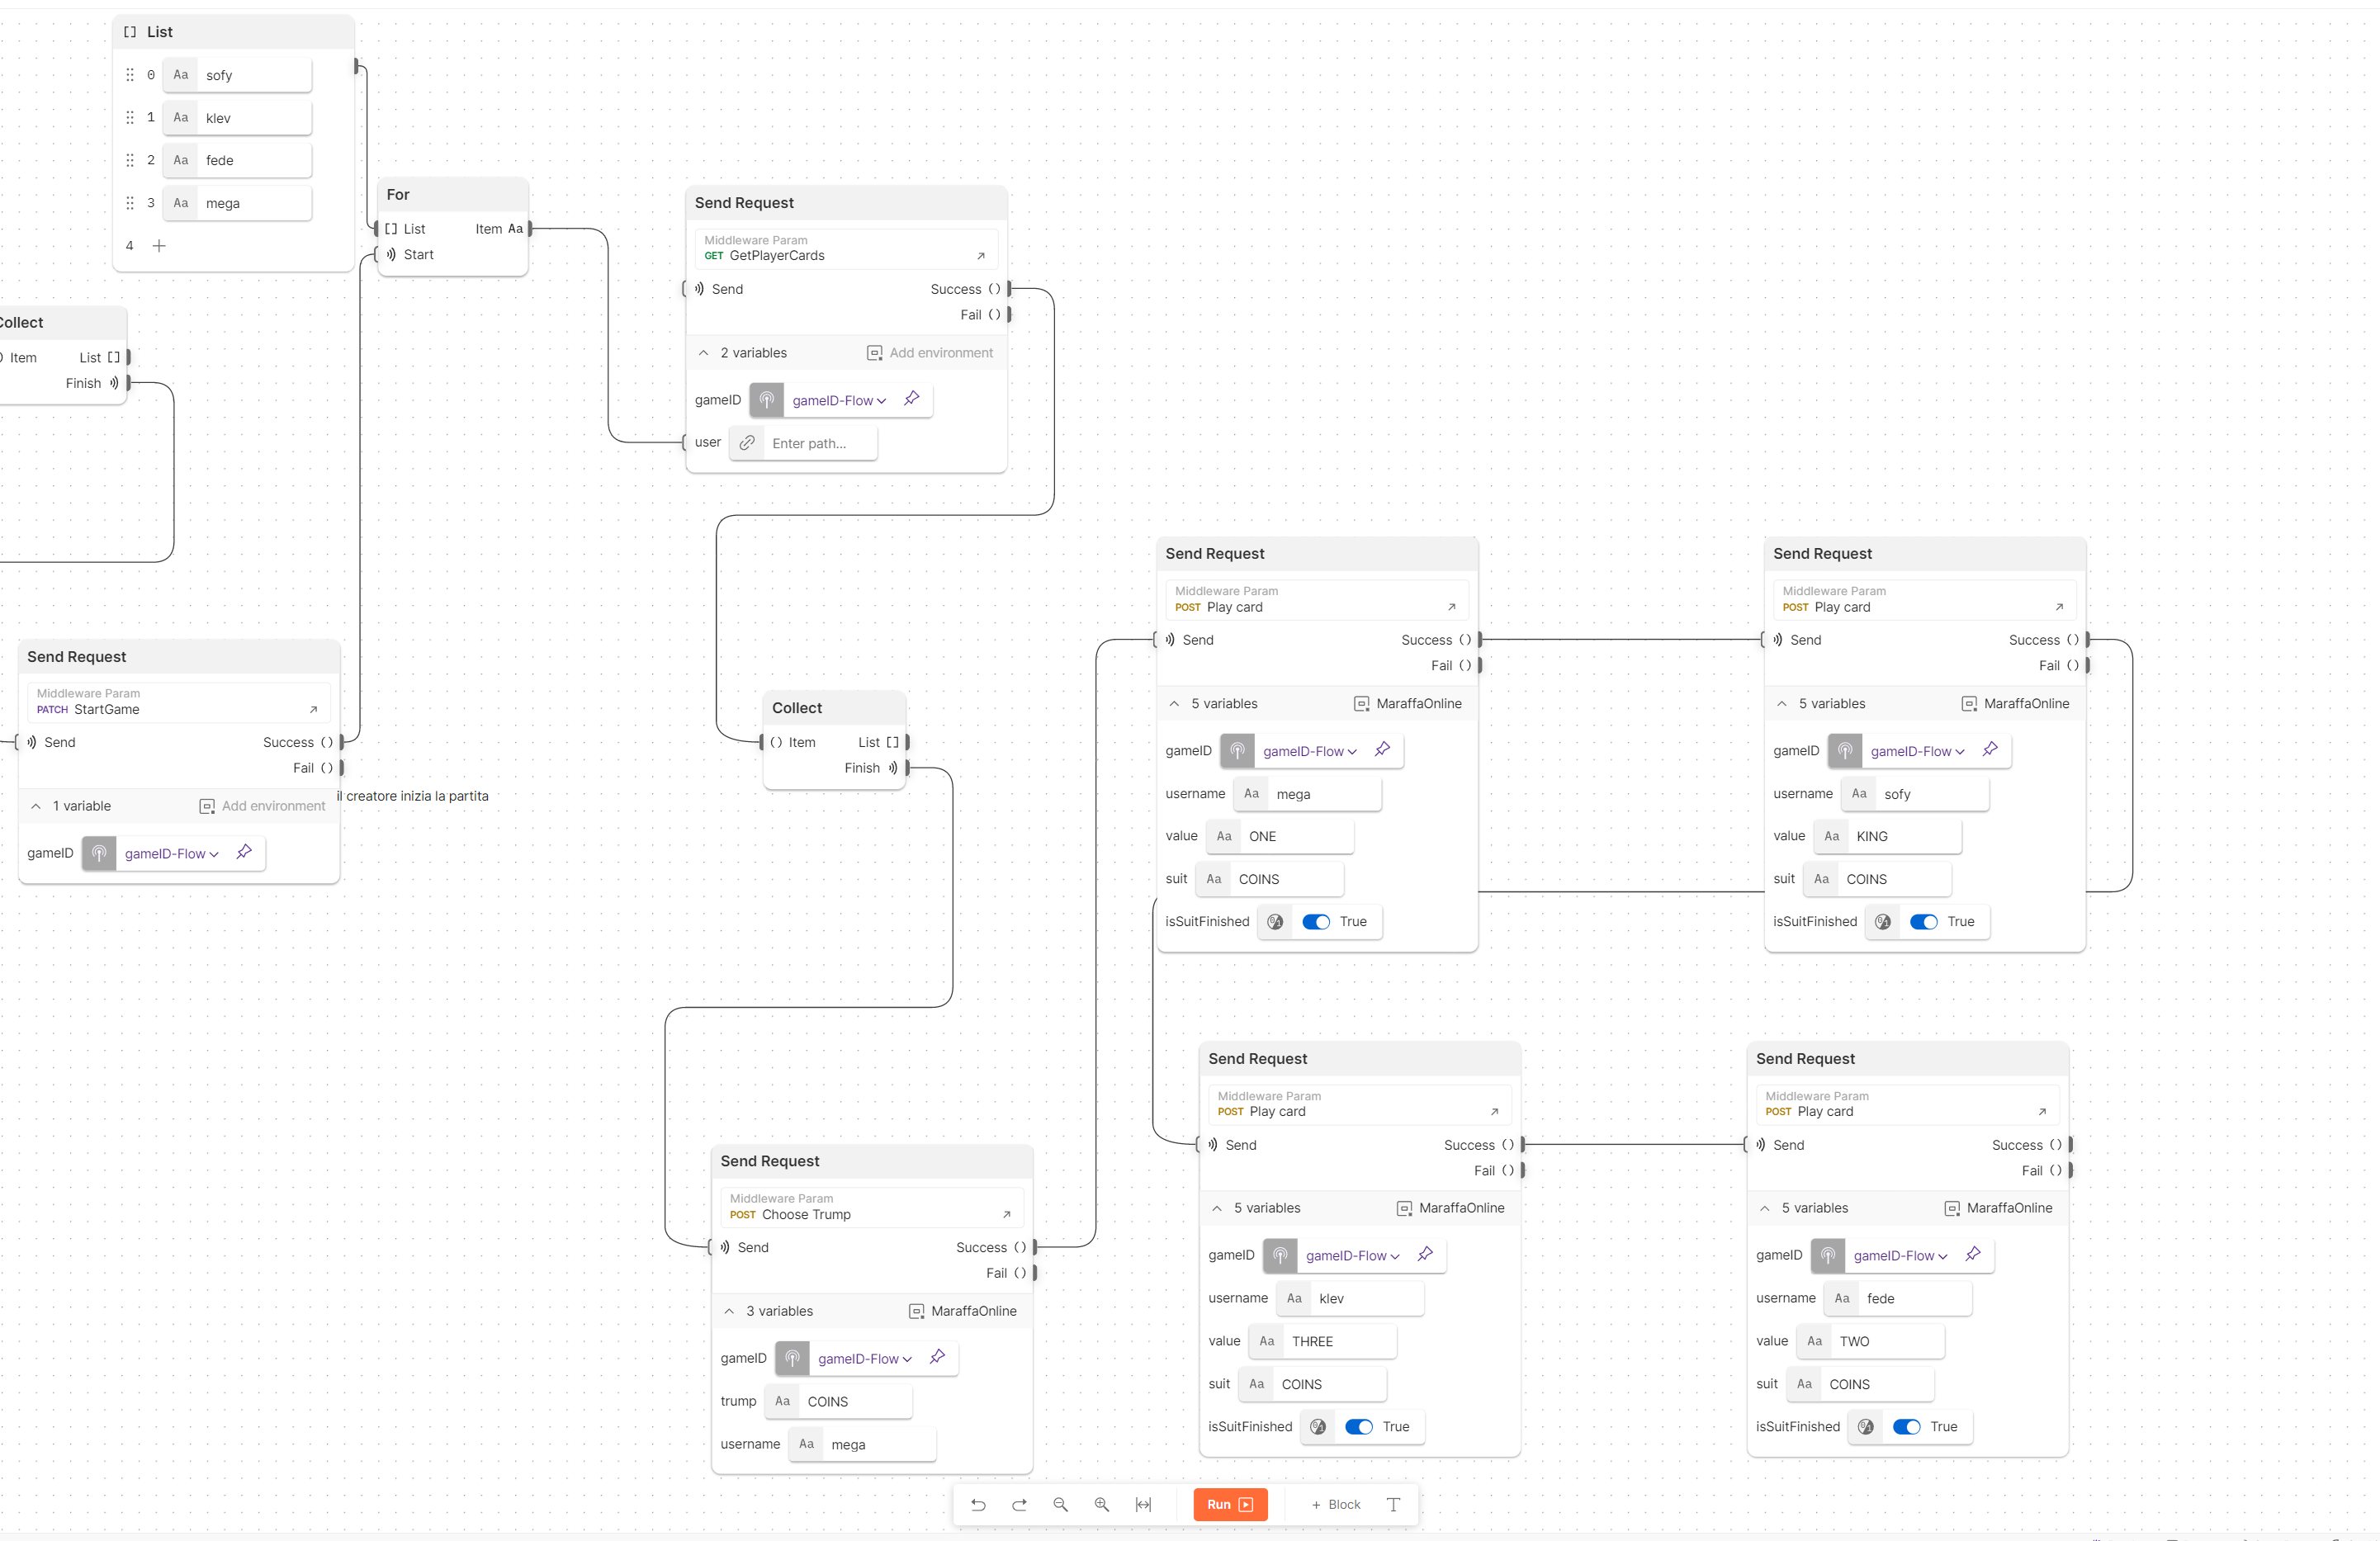
\includegraphics[width=18cm, height=10cm]{report/img/postManFlow.png}\\[7.5cm]


\subsection{Log automatici}

Il servizio core del sistema è il middleware e per poterlo monitorare è stato necessario implementare un sistema di log automatici. Tenere traccia di tutte le operazioni è un compito molto complesso e avrebbe reso difficile un eventuale debug su un software in produzione che in caso di errore potrebbe riavviarsi e perdere definitivamente quell'errore.
Grazie a Vertx, che offre "gratuitamente" un logger, e alla libreria \href{https://mvnrepository.com/artifact/ch.qos.logback/logback-classic}{\underline{LogBack}}, i log legati alle funzionalità più importanti sono trascritti su file .log in modo da poterli analizzare in caso di problemi.

Questo sistema poi si è evoluto grazie a una configurazione di LogBack in un file XML, tramite il quale è possibile personalizzare completamente il sistema di log, decidendo quali package loggare, in quali file trascriverli, scegliere il livello di log (info, debug, error, ecc.) e attuare un sistema di log rotate. Secondo questa configurazione, i log oltre una certa dimensione vengono compressi e rinominati per non occupare troppo spazio, e si può anche impostare il numero di questi file compressi da mantenere.

\begin{lstlisting}[language=Xml, caption={File configurazione Log automatici}, label=list:xml_logback]
    <appender name="DEBUG_LOG" class="ch.qos.logback.core.rolling.RollingFileAppender">
        <file>${DEBUG_FILE}</file>
        <rollingPolicy class="ch.qos.logback.core.rolling.SizeAndTimeBasedRollingPolicy">
            <fileNamePattern>${DEBUG_FILE}.%d{yyyy-MM-dd}.%i.gz</fileNamePattern>
            <maxFileSize>900MB</maxFileSize>
            <maxHistory>14</maxHistory>
            <totalSizeCap>2GB</totalSizeCap>
        </rollingPolicy>
        <encoder>
            <pattern>${LOG_PATTERN}</pattern>
        </encoder>
    </appender>


    <!-- Il package game usera la configurazione del log di debug -->
    <logger level="INFO" name="game" additivity="false">
        <appender-ref ref="DEBUG_LOG_ASYNC"/>
    </logger>

\end{lstlisting}

\vspace{1cm}

Questo sistema si adatta perfettamente a un software dockerizzabile che ha montato un volume relativo alla cartella /log, che può anche essere un volume remoto, da cui è possibile consultare velocemente i log in caso di problemi.

\begin{lstlisting}[language=Python, caption={Volume di log nel dockerfile l.13 da montare successivamente}, label=list:dockerfile_log]
FROM gradle:8.6.0-jdk17 AS build
COPY --chown=gradle:gradle . /home/gradle/src
WORKDIR /home/gradle/src
RUN gradle assemble
RUN gradle fatJar 

FROM openjdk:19

RUN mkdir /app
RUN mkdir /app/log

COPY --from=build /home/gradle/src/app/build/libs/ /app/
COPY --from=build /home/gradle/src/app/log /app/log

EXPOSE 3003
ENTRYPOINT ["java","-jar","/app/Middleware.jar"]
\end{lstlisting}


\subsection{Lettura variabili d'ambiente}

Data la scelta di dockerizzare interamente i servizi, è stato necessario l'utilizzo di variabili d'ambiente. Questo ha permesso di creare un sistema di deploy molto flessibile, in cui è possibile cambiare l'indirizzo del servizio a cui connettersi semplicemente modificando il file di configurazione del Docker Compose. I servizi in NodeJS leggono il contenuto delle variabili d'ambiente tramite il modulo `process.env`, mentre i servizi in Java utilizzano `System.getenv`. Questi comportamenti sono corretti per lo sviluppo locale e per ambienti di produzione in cui le variabili d'ambiente sono settate correttamente.

Per quanto riguarda invece lo sviluppo in CI, è stato necessario creare un file `.env.example` che contenesse tutte le variabili d'ambiente necessarie al funzionamento del servizio, in modo da poterle settare correttamente nel CI/CD, soprattutto per la fase di testing, e metterlo sulla repository. È importante tenere a mente che non dovrebbero mai essere caricati dati sensibili su strumenti di controllo di versione. In questo caso, non ci sono database o account cloud eventualmente raggiungibili dall'esterno.
    
\chapter{DevOps}
\label{ch:DevOps} % Label for method chapter
\section{Semantic Versioning, changelog e secrets}
\subsection{Semantic Versioning}
Per ogni release è stato adottato il semanting Versioning. È stato utilizzato il formato X.Y.Z, partendo da 1.0.0, ogni release incrementa il numero di versione in base a:
\begin{itemize}
    \item \textbf{Major (X):} per cambiamenti incompatibili con le versioni precedenti
    \item \textbf{Minor (Y):} per aggiunta di nuove funzionalità compatibili con le versioni precedenti
    \item \textbf{Patch (Z):} per correzione di bug compatibili con le versioni precedenti
\end{itemize}
Per ogni release viene creato anche un tag con la corrispondente versione.
\subsection{Changelog e secrets}
Ogni volta che is effettua una push sul main, viene generato un changelog. Il changelog è un file che contiene tutte le modifiche effettuate.
Nel changelog vengono riportati ogni commit che indicano le modifiche apportate, i contributori e il codice sorgente.
Se presenti, vengono inoltre riportate le sezioni: 
\begin{itemize}
    \item \textbf{feat: Feature} per le nuove funzionalità
    \item \textbf{fix: Bug Fixes} per le correzioni di bug
    \item \textbf{docs: Documentation} per le modifiche alla documentazione
    \item \textbf{refactor: Refactor} per le modifiche al codice che non aggiungono nuove funzionalità
    \item \textbf{perf: Performance Improvements} per le modifiche che migliorano le prestazioni
    \item \textbf{CI: Continuos Integration} per le modifiche alla CI
\end{itemize}
Il changelog viene autogenerato tramite l'action 'BobAnkh/auto-generate-changelog@v1.2.5'.
Inoltre per evitare un accesso non autorizzato a dati sensibili, come l'access token del changelog, sono stati inseriti in secrets, variabili d'ambiente di Github. 
\section{Licensing e issue template}
In ogni nostra repo è presente una licenza MIT. È stata scelta questa licenza perché è estremamente permissiva: 
il codice sorgente di Maraffa Online è open source e pertanto gli utenti possono utilizzarlo, modificarlo e distribuirlo.
Inoltre la licenza MIT è compatibile anche con altre licenze, anche con quelle restrittive come GPL.
È incoraggiata la collaborazione anche grazie alla presenza di un template con il quale un utente può consigliare nuove feature,
 segnalare un bug o suggerire un'implementazione alternativa.
\section{DVCS}

Come strumento di controllo di versione è stato scelto git, sono state adottate le seguenti best practices o git policy per garantire un flusso di lavoro coerente e prevenire conflitti di merge.
% La Git Policy rappresenta un insieme di linee guida e regole che governano l'uso di Git all'interno di un team di sviluppo. 
% Queste politiche sono fondamentali per garantire un flusso di lavoro coerente, prevenire conflitti di merge e mantenere una storia del codice chiara e facilmente navigabile. 

\subsection{Struttura dei Branch}

Una delle componenti principali della Git Policy è la gestione dei branch. La struttura tipica prevede almeno tre tipi di branch:
\begin{itemize}
 \item \textbf{Master/Main:} Questo è il branch principale che contiene il codice di produzione. Ogni commit su questo branch dovrebbe essere stabile e pronto per il rilascio. Questo branch e stato protetto per evitare commit diretti, richiedendo quindi una revisione per ogni operazione di merge.
 \item \textbf{Develop:} Qui viene integrato il lavoro di sviluppo corrente. È il branch dove confluiscono le feature prima di essere preparate per il rilascio. Questo branch dovrebbe essere costantemente aggiornato e testato per assicurare che sia in uno stato pronto per la produzione.
 \item \textbf{Feature Branches:} Utilizzati per lo sviluppo di nuove funzionalità. Ogni feature branch deve derivare da `develop` e, una volta completata la feature, viene reintegrato in `develop` tramite una pull request.
\end{itemize}


% \subsection{Commit e Messaggi di Commit}

% La pratica adottata per i commit è stata quella di effettuare commit frequenti e significativi.
% Per facilitare la comprensione di ogni commit si è adotatto lo standard : \href{https://www.conventionalcommits.org/en/v1.0.0/}{Conventional Commits}, che divide i commit in categorie come `fix`, `feat`, `docs`, `style`, `refactor`, `test`, `chore`, `ci`, `perf`, `build`, `revert`. 

\subsection{Pull Request e Code Review}

Le pull request (PR) sono essenziali per garantire la qualità del codice. Ogni PR è stata sottoposta a una code review da parte di uno o più membri del team. 
Questo processo non solo aiuta a individuare errori e problemi di design, ma promuove anche la condivisione delle conoscenze e facilita, tramite la 
comparazione di codice, la spiegazione di nuove funzionalità introdotte entro la fine dello sprint.


\subsection{Gestione dei Conflitti}

I conflitti di merge sono inevitabili in un ambiente di sviluppo collaborativo soprattutto quando è difficile modulare le parti di un SW.
% La gestione di confilitti, è stata gestita preferendo la risoluzione locale, in modo da evitare conflitti complessi e blocchi nel flusso di lavoro.
La scelta tra merge e rebase è stata fatta in base al contesto e alla complessità delle modifiche, privilegiando la chiarezza della storia del codice seppur a discapito della linearità, 
quindi di utilizzare il merge per mantenere una storia del codice più pulita e continua.
Questo è particolarmente utile per tracciare
l’evoluzione del progetto e per individuare facilmente l’origine dei bug. 
Infatti con il rebase c'è il rischio che venga cancellata una parte della history. In alcuni casi, può risultare molto pericoloso e 
può introdurre rischi significativi se non utilizzato con estrema cautela:
ipotizzando di introdurre un bug e successivamente di eseguire il rebase che cancella dalla history la modifica che ha introdotto il bug,
risulterebbe particolarmente ostico tracciare le modifiche e risalire a questo cambiamento. Potenzialmente può creare anche confusione tra i membri del team.

% Infatti, il merge evita 
% di riscrivere la cronologia dei commit, il che può causare problemi se altri sviluppatori hanno 
% basato il loro lavoro sui commit riscritti.  il rebase può introdurre rischi significativi se non utilizzato con estrema cautela
% in quanto riscrive la cronologia, rendendo difficile tracciare le modifiche originarie e potenzialmente causando confusione tra i membri del team.

% \subsection{Gestione dei conflitti in Git e scelta della tattica di merge}

% La gestione dei conflitti in Git è una parte fondamentale del flusso di lavoro collaborativo. I conflitti si verificano quando due o più branch presentano modifiche incompatibili agli stessi file o alle stesse righe di codice. Per risolvere questi conflitti, Git offre due principali tattiche: merge e rebase.

% Il merge è generalmente preferito al rebase in molti contesti di team per diversi motivi. Innanzitutto, il merge preserva la cronologia completa del progetto, mantenendo un registro di tutte le modifiche e delle fusioni effettuate. Questo è particolarmente utile per tracciare l'evoluzione del progetto e per individuare facilmente l'origine dei bug. Inoltre, il merge evita di riscrivere la cronologia dei commit, il che può causare problemi se altri sviluppatori hanno basato il loro lavoro sui commit riscritti. 

% Il rebase, sebbene utile per mantenere una cronologia lineare e pulita, può complicare la risoluzione dei conflitti in quanto riscrive la cronologia, rendendo difficile tracciare le modifiche originarie e potenzialmente causando confusione tra i membri del team. In ambienti collaborativi, il rebase può introdurre rischi significativi se non utilizzato con estrema cautela.

% In sintesi, mentre il rebase può essere utile in specifiche situazioni, il merge è solitamente preferito per la sua capacità di mantenere una cronologia trasparente e di evitare i problemi associati alla riscrittura della cronologia dei commit.


\subsection{Strumenti di Supporto TODO questo utile potrebbe essere spostato in un'altra sezione}

Per implementare efficacemente queste best practices, è utile utilizzare strumenti di supporto come:
- \textbf{Git Hooks:} Script che vengono eseguiti automaticamente in determinati punti del flusso di lavoro di Git, come prima di un commit o dopo un merge. Possono essere utilizzati per verificare la qualità del codice, eseguire test automatizzati, o applicare formattazioni standard.
- \textbf{Linting e Formattazione Automatizzata:} Utilizza strumenti come ESLint o Prettier per mantenere uno stile di codice coerente e rilevare potenziali errori prima che vengano committati.
- \textbf{Monitoraggio e Analisi:} Strumenti come SonarQube possono analizzare il codice per trovare problemi di sicurezza, bug, e debito tecnico.

% \subsection{Strategy for version control}
% **parla della git policy**
% \subsection{Git workflow}
% **main, develop, feature branch...***
\subsection{Commit verification}
È stato utilizzato il meccanismo di commit verification per assicurare:
\begin{itemize}
    \item \textbf{Integrità:} controllo sull'alterazione dei file presenti all'interno del commit.  Utilizzando una funzione hash, ci si assicura che non siano stati alterati in non modo autorizzato.
    \item \textbf{Autenticità:} controllo sull'autore del commit. Utilizzando una firma digitale, ci si assicura che il commit sia stato effettuato dall'autore autorizzato.
\end{itemize}
I controlli vengono effettuati in seguito a un merge. \\
Quando un commit è verificato viene prodotto un tag verde con la scritta "verified" e un tag rosso con la scritta "unverified" in caso contrario:
\begin{figure}[h!]
    \centering 
    
\includegraphics[scale=0.7]{report/img/verified_commit.png}
    \caption{Verified commit}
    \label{verified_commit}
    \end{figure}
\subsection{Conventional commits}
La pratica adottata per i commit è stata quella di effettuare commit frequenti e significativi.

In ogni repo è stato adottato un sistema standard per scrivere i commit:  i conventional commit. In questo modo i commit risultano più chiari e facilmente leggibili. 
Riportiamo di seguito la nomenclatura usata:
\begin{itemize}
    \item \textbf{fix:} per i commit che risolvono un bug
    \item \textbf{feat:} per i commit che aggiungono una nuova feature
    \item \textbf{refactor:} per i commit che migliorano il codice senza aggiungere nuove funzionalità
    \item \textbf{docs:} per i commit che riguardano la documentazione
    \item \textbf{style:} per i commit che riguardano la formattazione del codice
    \item \textbf{test:} per i commit che riguardano i test
    \item \textbf{ci:} per i commit che riguardano la Continuous Integration
\end{itemize}
Inoltre sono evidenziati i breaking changes per le modifiche non più compatibili con le versioni precedenti.
La stessa nomenclatura viene utilizzata anche nel changelog.

\section{Build automation}
\section{Continuous Integration}
Abbiamo deciso di implementare ogni servizio in una repository diversa. La repository fornita è un contenitore di tutte le singole repository dei servizi.
Per ogni repository è stata implementata una CI specifica. \\

\subsection{UserManagementMaraffa e BusinessLogic:} Essendo le due repository estremamente simili e avendo entrambe un ambiente in node.js, è stato implementato un workflow pressochè analogo. Questo workflow reagisce all'evento push sul main branch, e pull request sui branch main e develop 
e sono stati implementati 3 job: build, test e deploy.
Dopo una checkout iniziale (fetch-depth è 0 in quanto il changelog necessita di tutta la history dei commit), viene creata una cache per permettere ai job di comunicare tra loro. Successivamente alla build il sistema viene testato (in entrambi i casi viene usata l'action di yarn) e infine viene effettuato il deploy del servizio containerizzato se l'evento è una pull request con la quale viene svolto il merge e quando l'action è closed (non sta progredendo e quindi l'esecuzione non è in corso). Nel deploy viene effettuato il chekout, si configura il nome del progetto, si configura la versione della build. Se il commit viene effettuato sul main si configura il nome del tag e la versione a "LATEST", nel caso non fosse nel main viene configurata la versione a "develop". Infine si effettua il login al Github container registry, la build e la push dell'immagine sul registro. L'immagine viene configurata in modo parametrico con delle variabili d'ambiente e il nome viene trasformato in minuscolo. 

\subsection{MiddlewareMaraffa:} //TODO
push su main, pull request su main e develop
build e test se pullrequest.merge = true 

Parte finale 
\textbf{ChatServer:} Il servizio è sviluppato in un ambiente Java, pertanto dopo aver effettuato il checkout nel job build and test,  si effettua il set-up di Java (distribuzione: temurin, versione 20). Viene svolto il set-up di Gradle, in cui viene usata un'action per la build e creata una cache. Inoltre viene aggiunto un commento con un riassunto dei risultati dei job  alla pull request, il cui valore è impostato a "on-failure". Si noti che il suo valore di default è "never"; se fosse "always", si potrebbero verificare scenari indesiderati. Il riassunto dei risultati dei job risulta particolarmente utile: un utente che vuole esaminare la pull request riesce a comprendere lo stato dei job (se sono stati eseguiti correttamente oppure no) in modo leggibile e intuitivo. Successivamente si effettua il deploy del container di rabbitMQ se l'evento è una pull request oppure se è una push sul master o se la stringa con il riferimento a github contiene "tags/v". Infine se tutti il job da cui dipende (build-and-test) non è fallito e non è stato interrotto. Con l'istruzione run si verifica che non ci siano stati dei fallimenti nel job deploy and test.

\textbf{FrontendMaraffa:} //TODO
Sarebbe figo spiegare come i nostri workflow hanno ridotto i conflitti di integrazione, il rilevamento precoce di bug e i problemi di compatibilità.

\section{Automated quality assurance}
**code quality, testing, reporting**
\section{Automated delivery}
**automatizzare l'esecuzione iniziale del sistema con build.gradle che specifica come
il file deve compilare, gestire dip e configurare altri apetti del build process**
\section{Deployment}
è opzionale
\section{Containerization}
** docker image for each microservice, docker file
docker compose grouping containers and defining dependencies**

Data l'architettura del progetto in microservizi, usare Docker per creare un'immagine per ogni servizio è stata una scelta naturale. 
L'obiettivo finale è avere un sistema facilmente deployabile e scalabile, eseguibile velocemente in un ambiente generico, con uno stack di container Docker che racchiuda tutto il sistema.
Per fare ciò è stato necessario creare un Dockerfile per ogni servizio, in modo da poter creare un'immagine durante la fase di deploy della continuous integration.
\vspace{1cm}

La \textbf{strategia di containerizzazione} per tutte le immagini create è stata quella di utilizzare un'immagine base di Alpine, in modo da avere immagini leggere e veloci da scaricare. Per ridurre la dimensione delle immagini,
si è utilizzata un'immagine di sviluppo per compilare il codice e un'immagine di produzione per eseguire il codice compilato, copiando solo i file necessari.

\begin{figure}[H]
\caption{Comparazione tra le immagini multi-stage e le immagini tradizionali}
\centering
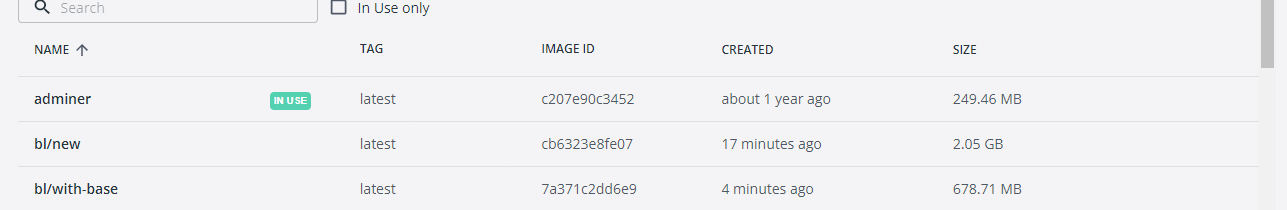
\includegraphics[width=12cm]{report/img/multi_stage.png}\\[10.5cm]
\end{figure}

\subsection{NodeJS}

I servizi UserManagementMaraffa e BusinessLogic sono stati containerizzati utilizzando un'immagine di Node.js. Nell'esempio sotto, si può notare la distinzione tra i diversi stage.
\vspace{1cm}

\begin{lstlisting}[language=Python, caption={Dockerfile delle immagini NodeJS}, label=list:dockerfile_nodejs]
FROM node:20-alpine as base
WORKDIR /app
COPY yarn.lock package.json /app/
RUN yarn install
COPY . /app
RUN yarn build

FROM node:20-alpine
WORKDIR /app    
COPY --from=base /app/package.json /app/package.json
COPY --from=base /app/node_modules /app/node_modules
COPY --from=base /app/dist /app/dist
EXPOSE 3000
CMD ["node","dist/main.js"]
\end{lstlisting}

\subsection{Java}

La containerizzazione del middleware ha richiesto alcuni passaggi aggiuntivi rispetto ai servizi in Node.js.
È stato necessario adottare immagini diverse per gli stage di build e produzione, quindi usare un'immagine di Gradle per la build, nella quale eseguire i comandi di Gradle, e un'immagine di 
OpenJDK per l'esecuzione del JAR prodotto dalla build.

Per la compilazione con Gradle, nonostante non sia una pratica corretta, è stato necessario mantenere nella repository il file gradle-wrapper.jar, in quanto non era possibile scaricarlo durante la build all'interno delle GitHub Actions.
La build non utilizza il classico comando di Gradle per generare il file .jar, ma un task personalizzato che si occupa di generare il fatJar del servizio, poiché le dipendenze non venivano gestite correttamente all'interno del normale file .jar.

\begin{lstlisting}[language=Java, caption={Task del fatJar da includere nel container}, label=list:gradle_fatJar]
tasks.register<Jar>("fatJar") {
    archiveBaseName.set("Middleware")
    manifest {
        attributes["Main-Class"] = "server.Main"
    }
    from(sourceSets.main.get().output)
    dependsOn(configurations.runtimeClasspath)
    from({ configurations.runtimeClasspath.get().filter { it.name.endsWith("jar") }.map { zipTree(it) } })
    dependsOn("compileJava")
    duplicatesStrategy = DuplicatesStrategy.EXCLUDE // Puoi utilizzare altre strategie come DuplicatesStrategy.WARN per avvisare ma non fermare la build
}
\end{lstlisting}

\subsection{Angular}

La containerizzazione del frontend ha richiesto l'utilizzo di un'immagine di Node.js per lo stage di build, mentre per l'esecuzione è stata utilizzata un'immagine di Nginx.
Nginx serve per eseguire l'applicazione all'interno del container e per poterla raggiungere dall'esterno. Per fare ciò è stato necessario configurare Nginx tramite un file di configurazione che ha permesso anche di gestire un'operazione di reverse proxy per indirizzare le chiamate al backend.

\begin{lstlisting}[language=Python, caption={Configurazione Nginx del front-end}, label=list:nginx_frontend]
server {
    listen 80;
    
    location / {
        root /usr/share/nginx/html;
        index index.html index.htm;
        try_files $uri $uri/ /index.html;
    }

    location /api/ {
        proxy_pass "http://${API_HOST}:${API_PORT}/";
        proxy_http_version 1.1;
        proxy_set_header Upgrade $http_upgrade;
        proxy_set_header Connection 'upgrade';
        proxy_set_header Host $host;
        proxy_cache_bypass $http_upgrade;
    }
}
\end{lstlisting}

L'indirizzo del backend è stato configurato tramite variabili d'ambiente, in modo da poterlo cambiare facilmente in base all'ambiente in cui si trova il container, e queste variabili vengono sostituite a seconda dell'ambiente di deploy in cui l'applicativo Angular viene eseguito.


\section{Docker-compose TODO}
TODO quando potremo testare un po'meglio e essere sicuri che effettivamente funzioni


% We mentioned in Chapter~\ref{ch:into} %[example backward reference to a chapter or section.]
% that a project report's structure could follow a particular paradigm. Hence, the organization of a report (effectively the Table of Content of a report) can vary depending on the type of project you are doing. Check which of the given examples suit your project. Alternatively, follow your supervisor's advice.

% \section{Examples of the sections of a methodology chapter}
% A general report structure is summarised (suggested) in Table~\ref{tab:gen_template}. Table~\ref{tab:gen_template} describes that, in general, a typical report structure has three main parts: (1) front matter, (2) main text, and (3) end matter. %[\textbf{also notice that the preceding sentence is an example of a numbered list in a text body}]. 
% The structure of the front matter and end matter will remain the same for all the undergraduate final year project report. However, the main text varies as per the project's needs.
% \begin{table}[h!]
%     \centering
%     \caption{Undergraduate report template structure}
%     \label{tab:gen_template}
%     \begin{tabular}{llll}     
%         \toprule
%         \multirow{7}{3cm}{Frontmatter} 
%         & & Title Page & \\                  
%         & & Abstract &    \\          
%         & & Acknowledgements & \\                            
%         & & Table of Contents &    \\                                
%         & & List of Figures   &    \\                        
%         & & List of Tables    &    \\                
%         & & List of Abbreviations  &    \\                     
%         & &   &    \\                        
%         \multirow{7}{3cm}{Main text}
%         & Chapter 1 & Introduction   &    \\                         
%         & Chapter 2 & Literature Review   &    \\
%         & Chapter 3 & Methodology   &    \\
%         & Chapter 4 & Results    &    \\
%         & Chapter 5 & Discussion and Analysis  &    \\
%         & Chapter 6 & Conclusions and Future Work  &    \\        
%         & Chapter 7 & Refection  &    \\          
%         & &   &    \\                       
%         \multirow{2}{3cm}{End matter}
%         & & References  &    \\   
%         & & Appendices (Optional)  &    \\ 
%         & & Index (Optional)  &    \\ 
%         \bottomrule
%     \end{tabular}
% \end{table}

% \subsection{Example of a software/Web development main text structure}
% \label{subsec:se_chpters}
% Notice that the ``methodology'' Chapter of Software/Web development in Table~\ref{tab:soft_eng_temp} takes a standard software engineering paradigm (approach). Alternatively, these suggested sections can be the chapters of their own. Also, notice that ``Chapter 5'' in Table~\ref{tab:soft_eng_temp} is ``Testing and Validation'' which is different from the general report template mentioned in Table~\ref{tab:gen_template}. Check with your supervisor if in doubt.
% \begin{table}[h!]
%     \centering
%     \caption{Example of a software engineering-type report structure}
%     \label{tab:soft_eng_temp}
%     \begin{tabular}{lll}     
%         \toprule                   
%         Chapter 1 & Introduction   &    \\        
%         Chapter 2 & Literature Review  &    \\                   
%         Chapter 3 & Methodology   &    \\
%         &               & Requirements specifications   \\
%         &               & Analysis   \\
%         &               & Design   \\
%         &               & Implementations   \\
%         Chapter 4 & Testing and Validation  &    \\
%         Chapter 5 & Results and Discussion      &    \\
%         Chapter 6 & Conclusions and Future Work  &    \\        
%         Chapter 7 & Reflection  &    \\                          
%         \bottomrule
%     \end{tabular}
% \end{table}

% \subsection{Example of an algorithm analysis main text structure}
% Some project might involve the implementation of a state-of-the-art algorithm and its performance analysis and comparison with other algorithms. In that case, the suggestion in Table~\ref{tab:algo_temp} may suit you the best. 
% \begin{table}[h!]
%     \centering
%     \caption{Example of an algorithm analysis type report structure}
%     \label{tab:algo_temp}
%     \begin{tabular}{lll}     
%         \toprule                   
%         Chapter 1 & Introduction  &    \\        
%         Chapter 2 & Literature Review  &    \\                
%         Chapter 3 & Methodology   &    \\
%         &               & Algorithms descriptions  \\
%         &               & Implementations   \\
%         &               & Experiments design   \\
%         Chapter 4 & Results       &  \\
%         Chapter 5 & Discussion and Analysis  &    \\
%         Chapter 6 & Conclusion and Future Work  &    \\        
%         Chapter 7 & Reflection  &    \\          
%         \bottomrule
%     \end{tabular}
% \end{table}

% \subsection{Example of an application type main text structure}
% If you are applying some algorithms/tools/technologies on some problems/datasets/etc., you may use the methodology section prescribed in Table~\ref{tab:app_temp}.  
% \begin{table}[h!]
%     \centering
%     \caption{Example of an application type report structure}
%     \label{tab:app_temp}
%     \begin{tabular}{lll}     
%         \toprule                   
%         Chapter 1 & Introduction  &    \\        
%         Chapter 2 & Literature Review  &    \\                
%         Chapter 3 & Methodology   &    \\
%         &               & Problems (tasks) descriptions  \\
%         &               & Algorithms/tools/technologies/etc. descriptions  \\        
%         &               & Implementations   \\
%         &               & Experiments design and setup   \\
%         Chapter 4 & Results       &  \\
%         Chapter 5 & Discussion and Analysis  &    \\
%         Chapter 6 & Conclusion and Future Work  &    \\        
%         Chapter 7 & Reflection  &    \\          
%         \bottomrule
%     \end{tabular}
% \end{table}

% \subsection{Example of a science lab-type main text structure}
% If you are doing a science lab experiment type of project, you may use the  methodology section suggested in Table~\ref{tab:lab_temp}. In this kind of project, you may refer to the ``Methodology'' section as ``Materials and Methods.''
% \begin{table}[h!]
%     \centering
%     \caption{Example of a science lab experiment-type report structure}
%     \label{tab:lab_temp}
%     \begin{tabular}{lll}     
%         \toprule                   
%         Chapter 1 & Introduction  &    \\        
%         Chapter 2 & Literature Review  &    \\                
%         Chapter 3 & Materials and Methods   &    \\
%         &               & Problems (tasks) description  \\
%         &               & Materials \\        
%         &               & Procedures  \\                
%         &               & Implementations   \\
%         &               & Experiment set-up   \\
%         Chapter 4 & Results       &  \\
%         Chapter 5 & Discussion and Analysis  &    \\
%         Chapter 6 & Conclusion and Future Work  &    \\        
%         Chapter 7 & Reflection  &    \\          
%         \bottomrule
%     \end{tabular}
% \end{table}

% \section{Example of an Equation in \LaTeX}
% Eq.~\ref{eq:eq_example} [note that this is an example of an equation's in-text citation] is an example of an equation in \LaTeX. In Eq.~\eqref{eq:eq_example}, $ s $ is the mean of elements $ x_i \in \mathbf{x} $: 

% \begin{equation}
% \label{eq:eq_example} % label used to refer the eq in text
% s = \frac{1}{N} \sum_{i = 1}^{N} x_i. 
% \end{equation}

% Have you noticed that all the variables of the equation are defined using the \textbf{in-text} maths command \$.\$, and Eq.~\eqref{eq:eq_example} is treated as a part of the sentence with proper punctuation? Always treat an equation or expression as a part of the sentence. 

% \section{Example of a Figure in \LaTeX}
% Figure~\ref{fig:chart_a} is an example of a figure in \LaTeX. For more details, check the link:

% \href{https://en.wikibooks.org/wiki/LaTeX/Floats,_Figures_and_Captions}{wikibooks.org/wiki/LaTeX/Floats,\_Figures\_and\_Captions}.

% \noindent
% Keep your artwork (graphics, figures, illustrations) clean and readable. At least 300dpi is a good resolution of a PNG format artwork. However, an SVG format artwork saved as a PDF will produce the best quality graphics. There are numerous tools out there that can produce vector graphics and let you save that as an SVG file and/or as a PDF file. One example of such a tool is the ``Flow algorithm software''. Here is the link for that: \href{http://www.flowgorithm.org/download/}{flowgorithm.org}.
% \begin{figure}[ht]
%     \centering
%     % \includegraphics[scale=0.3]{figures/chart.pdf}
%     \caption{Example figure in \LaTeX.}
%     \label{fig:chart_a}
% \end{figure}

% \clearpage %  use command \clearpage when you want section or text to appear in the next page.

% \section{Example of an algorithm in \LaTeX}
% Algorithm~\ref{algo:algo_example} is a good example of an algorithm in \LaTeX.  
% \begin{algorithm}
%     \caption{Example caption: sum of all even numbers}
%     \label{algo:algo_example}
%     \begin{algorithmic}[1]
%         \Require{$ \mathbf{x}  = x_1, x_2, \ldots, x_N$}
%         \Ensure{$EvenSum$ (Sum of even numbers in $ \mathbf{x} $)}
%         \Statex
%         \Function{EvenSummation}{$\mathbf{x}$}
%         \State {$EvenSum$ $\gets$ {$0$}}
%         \State {$N$ $\gets$ {$length(\mathbf{x})$}}
%         \For{$i \gets 1$ to $N$}                    
%         \If{$ x_i\mod 2 == 0$}  \Comment check if a number is even?
%         \State {$EvenSum$ $\gets$ {$EvenSum + x_i$}}
%         \EndIf
%         \EndFor
%         \State \Return {$EvenSum$}
%         \EndFunction
%     \end{algorithmic}
% \end{algorithm}
 
% \section{Example of code snippet  in \LaTeX}

% Code Listing~\ref{list:python_code_ex} is a good example of including a code snippet in a report. While using code snippets, take care of the following:
% \begin{itemize}
%     \item do not paste your entire code (implementation) or everything you have coded. Add code snippets only. 
%     \item The algorithm shown in Algorithm~\ref{algo:algo_example} is usually preferred over code snippets in a technical/scientific report. 
%     \item Make sure the entire code snippet or algorithm stays on a single page and does not overflow to another page(s).  
% \end{itemize}

% Here are three examples of code snippets for three different languages (Python, Java, and CPP) illustrated in Listings~\ref{list:python_code_ex}, \ref{list:java_code_ex}, and \ref{list:cpp_code_ex} respectively.  

% \begin{lstlisting}[language=Python, caption={Code snippet in \LaTeX ~and  this is a Python code example}, label=list:python_code_ex]
% import numpy as np

% x  = [0, 1, 2, 3, 4, 5] # assign values to an array
% evenSum = evenSummation(x) # call a function

% def evenSummation(x):
%     evenSum = 0
%     n = len(x)
%     for i in range(n):
%         if np.mod(x[i],2) == 0: # check if a number is even?
%             evenSum = evenSum + x[i]
%     return evenSum
% \end{lstlisting}

% Here we used  the ``\textbackslash clearpage'' command and forced-out the second listing example onto the next page. 
% \clearpage  %
% \begin{lstlisting}[language=Java, caption={Code snippet in \LaTeX ~and  this is a Java code example}, label=list:java_code_ex]
% public class EvenSum{ 
%     public static int evenSummation(int[] x){
%         int evenSum = 0;
%         int n = x.length;
%         for(int i = 0; i < n; i++){
%             if(x[i]%2 == 0){ // check if a number is even?
%                 evenSum = evenSum + x[i];
%             }
%         }
%         return evenSum;     
%     }
%     public static void main(String[] args){ 
%         int[] x  = {0, 1, 2, 3, 4, 5}; // assign values to an array
%         int evenSum = evenSummation(x);
%         System.out.println(evenSum);
%     } 
% } 
% \end{lstlisting}


% \begin{lstlisting}[language=C, caption={Code snippet in \LaTeX ~and  this is a C/C++ code example}, label=list:cpp_code_ex]
% int evenSummation(int x[]){
%     int evenSum = 0;
%     int n = sizeof(x);
%     for(int i = 0; i < n; i++){
%         if(x[i]%2 == 0){ // check if a number is even?
%             evenSum = evenSum + x[i];
%     	}
%     }
%     return evenSum;     
% }

% int main(){
%     int x[]  = {0, 1, 2, 3, 4, 5}; // assign values to an array
%     int evenSum = evenSummation(x);
%     cout<<evenSum;
%     return 0;
% }
% \end{lstlisting}



% \section{Example of in-text citation style}
% \subsection{Example of the equations and illustrations placement and reference in the text}
% Make sure whenever you refer to the equations, tables, figures, algorithms,  and listings for the first time, they also appear (placed) somewhere on the same page or in the following page(s). Always make sure to refer to the equations, tables and figures used in the report. Do not leave them without an \textbf{in-text citation}. You can refer to equations, tables and figures more them once.

% \subsection{Example of the equations and illustrations style}
% Write \textbf{Eq.} with an uppercase ``Eq`` for an equation before using an equation number with (\textbackslash eqref\{.\}). Use ``Table'' to refer to a table, ``Figure'' to refer to a figure, ``Algorithm'' to refer to an algorithm and ``Listing'' to refer to listings (code snippets). Note that, we do not use the articles ``a,'' ``an,'' and ``the'' before the words Eq., Figure, Table, and Listing, but you may use an article for referring the words figure, table, etc. in general.

% For example, the sentence ``A report structure is shown in \textbf{the} Table~\ref{tab:gen_template}'' should be written as ``A report structure is shown \textbf{in} Table~\ref{tab:gen_template}.'' 
 

% \section{Summary}
% Write a summary of this chapter.

% ~\\[5em]
% \noindent
% {\huge\textbf{Note:}} In the case of \textbf{software engineering} project a Chapter ``\textbf{Testing and Validation}'' should precede the ``Results'' chapter. See Section~\ref{subsec:se_chpters} for report organization of such project. 


    \chapter{Conclusions and Future Work}
\label{ch:con}
\section{Conclusions}

**spiega che verrà messo online nel sitoweb **

**Replace with a description of the conclusions**


Typically a conclusions chapter first summarizes the investigated problem and its aims and objectives. It summaries the critical/significant/major findings/results about the aims and objectives that have been obtained by applying the key methods/implementations/experiment set-ups. A conclusions chapter draws a picture/outline of your project's central and the most signification contributions and achievements. 

A good conclusions summary could be approximately 300--500 words long, but this is just a recommendation.

A conclusions chapter followed by an abstract is the last things you write in your project report.

\section{Future work}
This section should refer to Chapter~\ref{ch:results} where the author has reflected their criticality about their own solution. The future work is then sensibly proposed in this section.

\textbf{Guidance on writing future work:} While working on a project, you gain experience and learn the potential of your project and its future works. Discuss the future work of the project in technical terms. This has to be based on what has not been yet achieved in comparison to what you had initially planned and what you have learned from the project. Describe to a reader what future work(s) can be started from the things you have completed. This includes identifying what has not been achieved and what could be achieved. 



A good future work summary could be approximately 300--500 words long, but this is just a recommendation.

    
\end{document}
